\documentclass[a4paper]{article}

\usepackage{graphicx}
\usepackage{setspace}
\usepackage{ulem}
\usepackage{fullpage}
\usepackage[top=2cm, bottom=4.5cm, left=2.5cm, right=2.5cm]{geometry}

\title{Astronomy Notes}
\author{Bingan Chen}


\begin{document}

\doublespacing

	\maketitle
	
	\tableofcontents
	
	\newpage
	\section{Lecture 1}
	Thats the first class.
	
	\newpage
	
	\section{Lecture 2 - History of Astronomy}
	
	Sun Dagger Petroglyph:
	\begin{center}
		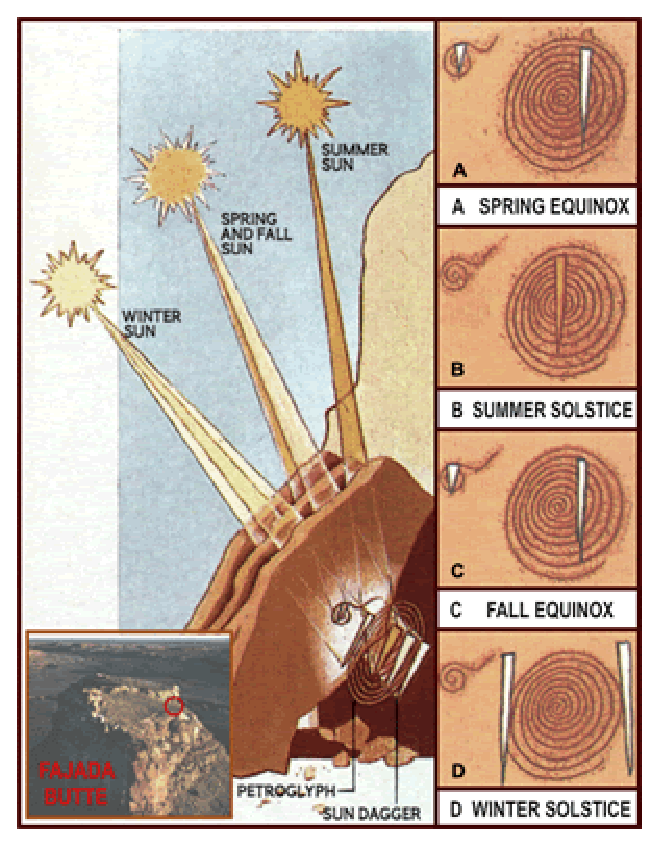
\includegraphics[scale=0.1]{001.eps}
		
	\end{center}
	
	Every human civilizations discover the astronomy.
	
	\subsection{Positions on the sky:}
	
	\textbf{Constellations} patterns of the apparent positions on the sky. All cultures are able to define the patterns cuz they won't change in a long period of time.\\
	
	There are movements of stars can be capture using long exposure. The point that doesn't move is called \textbf{Polaris} $\rightarrow$ caused by the rotation of the Earth.\\
	
	\subsection{Movement and Patterns of the Moon}
	The changing phases of the moon Every 27.3 ays or so, the Moon makes a complete revolution.
	
	Half of the moon is always illuminate by the Sun - but our view of its illuminated side changes $\rightarrow$ And the moon rotates at the same rates that rotates around the sun. \emph{Though we see the moon at the same side, its dark side always changes.}
	
	Because of the relative positions of moon with respect to Sun, the different phases can only be visible for certain period.
	
	Not all times the moon rise at the same place (due east but a bit north when coming to winter.)
	
	
	
	\subsection{Other patterns}
	The Sun moves with respect to background stars, so that at different times of the year you will see different constellation. 
	
	\textbf{This is due to the changing positions of the Earth in its orbit around the Sun.}
	
	\subsubsection{Eclipse}
	Will be discussed during Thursday.
	
	\section{Lecture 3-The Retrograde Motion}
	Venus and Jupiter also changes its positions.
	
	They sometimes moves back and forth, this motion calls retrograde motion.
	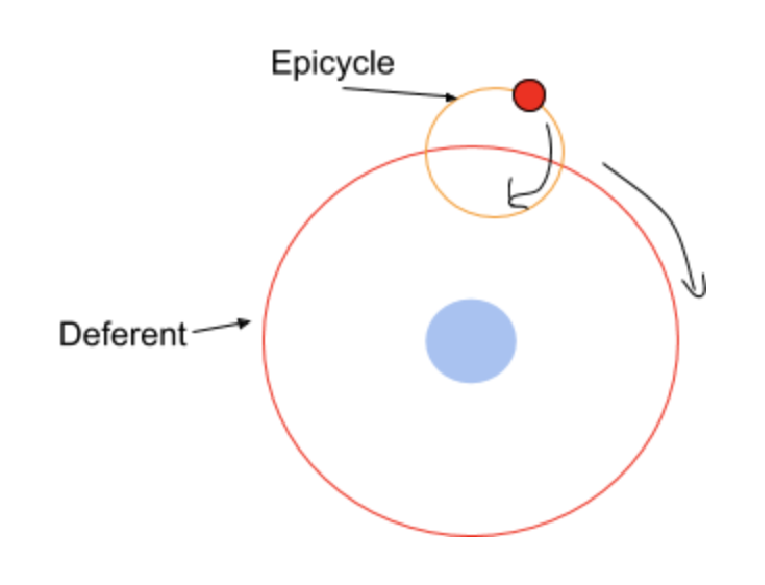
\includegraphics[scale=0.1]{002}
	
	When the Earth moving pass the Mars, there is a short period \emph{seems} like the Mars moves in an opposite way.
	
	Add sun and moon and there are 7 such things moving in the sky; Those match the 7 days of a weak.
	
	Aristotelian notions of physics includes for elements: Earth, water, air, and fire.
	
	The motions are mostly caused by the combined mass of a whole milky way.
	
	\section{Lecture 4}
	Around 150 AD, Greek people developed a simple \emph{geocentric model}.
	
	The \emph{parallactic motion} should be seen if the Earth were orbiting around the sun. (back-and-forth motion)
	
	In 1592, \emph{Galileo Galilei} accepted a position at the University of Padua where he would become well known for his work refuting basic tenets of Aristotle theory. He invented the telescope and proved that the Earth is not the center of all motions. Also the phases of \emph{Venus} and showed that \emph{Venus clearly had to be orbiting the sun}.
	\subsection{Kepler's Laws}
	\begin{itemize}
		\item Kepler was also refuting the traditional model. He paid attention to the planetary observations of Tycho Brahe to develop a series of laws of planetary motion.
		\item Kepler's 2nd law. Planet moves faster when they are closer to the sun, and slower when they are far.
		\item Kepler's 3rd law. The nearest moves faster and far moves slower (more on relationships).	
	\end{itemize}
	
	\subsection{Newton's Laws}
	Between 1665 and 1690, Newton discovered his theory about Speed, Velocity, and Acceleration.
	
	\section{Lecture 5 - Terrestrial and Jovian Planets}
	
	\emph{Today's lecture will be about the patterns of different planets.}
	
	The first pattern is one we've already seen, and was visible to even ancient astronomers - the planets all appear to orbit in the same general plane.
	
	This highly ordered arrangement makes it clear that the planets must have formed at roughly same time and in a way that had \emph{some preferred plane and axis} of rotation.
	
	The explanation about this phenomenon.
	
	We can see so much rotating disks of material. Many of them are clearly surrounded by disks of gas and dust. These flattened disks appear to be an inherent part of the formation of stars. The spinning shapes the cloud into a disk as it collapses because material in the equatorial plane has a harder time falling in to the center due to centrifugal accelerations. 
	
	As the solar nebula collapesd into a flatter, denser disk. the small material began to clump together or accrete, preserving the angular momentum just like the orbiting patterns as the formed from. \emph{This brings us the different planets in our solar system.}
	
	By the late 1800's it had become clear that the worlds of the outer Solar System were far different from those of the inner Solar System. Not only were these planets much farther apart from each other.
	
	The \textbf{Terrestrial Planets} are all Earthlike in that they share a similar internal structure. Their solid surfaces are all covered by a very thin later of gases and sometimes fluids. The composition, temperature and pressure are distinct. Those forces erase old craters and create new features on planetary surfaces. For moon and mercury have far less extensive atmospheres, this results in the little geographic change on surface since its formation.
	
	The \textbf{Jovian Planets} have much thicker atmosphere compared to terrestrial planets. They don't have the a solid surface at all underneath those bulky atmosphere. There deep interior are belieavedd to be composed if increasingly dense layers of hydrogen and hydrogen compounds, such as water, ammonia...
	
	\emph{Why are the Jovian planets so big?}\\
	The accretion process steadily built up all of the planets from solid, grain-sized particles (Similar to the meteorites we still see falling on the Earth.)	
	
	Near the forming sun, only rare heavy elements such as metals and rock could from such grains. Farther away from the forming stars, much more common hydrogen compounds like water vapor and methane were able to condense into ices.
	
	This allowed protoplanets in the other solar system to quickly grow larger - large enough for their gravity to begin attracting and holding on to hydrogen and helium gas, by far the most abundant materials in the Solar Nebula. 
	
	This \textbf{gas capture phase} helps explain much of this second pattern.
	
	The gravitational attraction of that infalling gas also brought some solid materials (some ices some rocks). 
	
	Ganymede is the largest moon in the Solar System.Jupiter raises powerful tides in its moon, and the huge mass tides produce frictional force that makes many heat inside the moon. Europa tidal heating may be just right to keep it to hold the liquid water. Titan is the most remarkable moons of Jupiter, because of the enormous atmosphere. 
	
	\section*{Discussion}
	Copernican Revolution(1550-1650)\\
	Gali Venus/Jupiter - Earth is not the center
	Kepler's second law: equal area / equal time - closer faster\\
	Kepler's third law: 
	\begin{equation}
		P^{2} \propto a^{3}
	\end{equation}
	While the equation is \(P^{2} = (M_1 + M_2) a^{3}\)	\\
	Newton's Universal Law of Gravitation:
	\begin{equation}
		F = G\frac{m_{1}m_{2}}{r^{2}}
	\end{equation}
	Remember the Kinds of planers.
	
	\section{Lecture 6-Astroids and Comets}
	
	The ring of Saturn was first discovered from Earth by Galileo.
	
	All jovian planets have ring system.
	
	The collision of their moons provide enough dust.
	
	Too small to be a spherical shape.
	
	\emph{Kuiper Belt} is a band of leftover planet-making material.
	\emph{Oort Cloud} used 
	
	\section{Lecture 7}
	The rings are believed to be created and replanished over time by collisions of asteroids and comets - mostly the latter - with the large moons of the Jovian planets. \\
	The majority of them have low inclinations\\
	The speed stars move depends upon the mass of the planet - more massive planets exert more gravitational forces.
	\\
	Another method for detecting planets around other stars is the so-called "transit method". \(\rightarrow\) get the radius.
	\\
	\emph{habitable zone} is really all about the possibility of \emph{liquid water on a planet's surface}. 
	
	\section*{Lecture 9-The stars}
	In order to see the small planets around the large stars, a big telecscope is needed. \\
	Man made light are \emph{reflected} by the atmosphere.\emph{Light polution} is the major reason why \\
	astronomers put large telescopes in remote locations.\\ Also, turbulence in the atmosphere also \emph{distort} light, making stars appear to twinkle in color. 
	The apparent jiggling of the stars. \textbf{This can be fixed by some adaptive optices.} The light wave can be restored.\\
	However, the most severe problem caused by the atmosphere is the \emph{absorption} of light. It absorb most of the light.
	Some details cannot be captured without infrared. \textbf{That's why we put our telescope in the space.} (not because they are closer to the stars)\\
	\textbf{William Herschel} discoverd Uranus and found the non-visible light.\\
	\subsection*{The sun}
	We know how the sun really works is\dots
	These are what we can measure:
	\begin{itemize}
		\item how bright stars appear to be as seen from Earth.
		\item how much and in what diretions they are moving.
		\item their color (or more precisely, their \emph{Spectural Energy Distribution} - how much UV vs. Visible vs. Radio
		\item Which absorption / emission lines are presnet in theiir spectra.
	\end{itemize}
	\underline{Luminosity} - the total amount of power radiated by a star into space, as measure at some fixed distance from the stars.
	\underline{Apparent Bright} - How we see on the Earth.
	\\The relationship is:
	\[ App\space Light = \frac{L}{4\pi d^{2}}\]
	If we could find either the luminosity and distance. \\
	We can use parallax to measure the distance using the parallax angle.\\
	To measure the \emph{luminosity} directly.  To measure the mass of stars, we can do it by directly observing the effect the gravity from another star.
	\\ Binary system can be used to find the \emph{radius} of a stars in systems that actually \emph{eclipse} each other.\\
	The luminosity is using the equation
	\[L = 4\pi R^2 \sigma T^4\]
	How could we precisely measure the temperature of a star?
	We could observe the \emph{absorption patterns}.\\
	It turns out that "spectral type" is not determined by a stars chemical composition. All stars contain 
	roughly 75\% H, 23\% He, and only 1-2\% of all the elements.

	\emph{Payne-Gaposechkin} showed that the temperature of a star's atmosphere dictates the type of ions or molecules that can exist there, and \\
	the energy states of electrons and atoms.
	\begin{center}
		\includegraphics[scale = 0.5]{SpectralLight.png}
	\end{center}
	In specific, \emph{M-type} stars dominate the univers.

	

\end{document}

